\documentclass[oribibl]{llncs}
\usepackage{amssymb,amsmath}
\usepackage{mathpartir}
\usepackage{verbatim}
\usepackage{saoithin}
\usepackage{tikz}
\usetikzlibrary{arrows,matrix}

%\def\PLAN#1{\textit{\textsf{{#1}}}}
\def\PLAN#1{}
\def\DRAFT#1{}
%\def\DRAFT#1{\textbf{DRAFT: }\textsf{{#1}}}



\title{
 The Logic of \UTP2
  \thanks{
    This research was supported by grants 07-RFP-CMSF186
    and 08-RFP-CMS1277 from Science Foundation Ireland, as well as partial support from
    Lero, the Irish Software Engineering Research Centre
  }
}

\author{%
Andrew Butterfield\inst{1}
}

\institute{%
Lero@TCD, Trinity College Dublin, \email{\{butrfeld\}@tcd.ie}
}


\bibliographystyle{alpha}

\input{UTP2LogicDefs}

\begin{document}

\maketitle

\begin{abstract}
\UTP2\ is a theorem prover developed to support the Unifying Theories
of Programming (UTP) framework.
Its primary design goal was to support the higher-order logic,
alphabets, equational reasoning and ``programs as predicates'' style
that is prevalent in much of the UTP literature,
from the seminal work by Hoare \& He onwards.
In this paper we focus on the matching engine that is the
heart of the theorem prover.
Designed to support the equational reaosning style of UTP,
as well as offering the flexibility of notation that is a hallmark
of much published UTP work, the law-matching process
involves structural matching merged with a blend of inference
systems that reason about types, side-conditions, and UTP's
own particular instance of the frame problem,
with regard to both alphabets and quantifier variable lists.
\end{abstract}


\section{Introduction}\label{sec:intro}

Unifying Theories of Programming (UTP) \cite{UTP-book},
is a framework that uses alphabetised predicates to define language
semantics in a relational calculus style, in a way that facilitates
the unification of otherwise disjoint semantic theories,
either by merging them, or using special linking predicates
that form a Galois connection. The framework is designed
to cover the spectrum from abstract specifications
all the way down to near-machine level descriptions,
and as a consequence the notion of refinement plays a key role.

In \cite{conf/utp/Butterfield10}
we gave an overview of the Unifying Theories of Programming Theorem Prover
(\UTP2)
that we are developing to support such theory development work%
\footnote{%
In that paper it was called \STHN, but the name has since changed to \UTP2
}%
.
The prover is an interactive tool, with a graphical user-interface,
designed to make it easy to define a UTP theory and to experiment
and perform the key foundational proofs.
The motivation for developing this tool,
rather than using an existing one has been discussed in some detail
in \cite{conf/utp/Butterfield10} and the  technical underpinning has been further elaborated upon in \cite{conf/utp/Butterfield12}.

Here we focus on a small subset of the logic and laws
in order to explain the key role of the extended matcher at the heart of \UTP2.
The focus is on the various matching and inference mechanisms and how they
interact to facilitate the application of laws in a proof at a level
that matches typical handwritten proof steps,
to the extent that this is feasible.

This paper assumes that the reader is familiar
with the basic ideas behind UTP, and does not give an introduction
to the subject. A good introduction is the key textbook written
by C.A.R. Hoare and He Jifeng \cite{UTP-book},
which is free to download from \texttt{unifyingtheories.org}.


\subsection{Matching: an overview}

The matching problem we consider in this paper can be summarised as follows:
during the course of a proof of some conjecture, we will have identified a sub-part
of the proof goal predicate that is of current interest---the \emph{target} focus predicate;
We will then indicate some collection of laws we hope might be applicable,
and then proceed to systematically match the target against those laws,
viewed as \emph{pattern} predicates.
The conjecture will have associated side-conditions,
as will each law---these are added to the match algorithm inputs.
A successful match returns a binding that maps all pattern variables
to the corresponding sub-parts of the target
($\pfun$ is a partial function arrow, while $\ffun$ is a finite partial function).
\[
match : (Pred\times Side) \fun (Pred\times Side) \pfun (Var \ffun \mbox{``Syntax''})
\]
Assuming some success, we can then choose from the range of successful matches,
and use this to apply the law.

In an equational reasoning system such as this, if we match a target
against a law successfully, then it is an instance of such a law,
hence universally true (this is what it means to be a law),
and so the only sensible replacement for the target is the constant predicate \True.
So, why do we return any bindings? Why not just a success/fail indicator?
There are two reasons, one algorithmic and pragmatic,
the other as a result of ensuring maximum flexibility
in the power of the prover:
\begin{enumerate}
  \item a match should fail if different sub-parts of the target
     match different sub-parts of the pattern, but with inconsistent bindings.
     So the attempt to merge these sub-bindings will uncover such problems.
  \item in an equational reasoning system, given law predicates of the
  forms $P \equiv Q$ or $P \implies Q$,
  it makes sense to try matches against either the lhs or rhs,
  with the other side viewed as a template for building the target replacement.
  The binding provides details of how the template should be instantiated.
\end{enumerate}
The process of
finding laws,
establishing if they have the special forms
just described,
 and working out the relevant replacement predicates
($\True$,or one of the law sides),
is fairly straightforward, and we do not discuss it further.

The real focus of this paper is on the function $match$ just introduced
above, and an exposition of how it is so much more than just an exercise
in structural template pattern-matching and merging the resulting bindings.

\subsection{Structure of this paper}

In Section \ref{sec:logic} we introduce a small subset of the logic of \UTP2,
and then in Section \ref{sec:variables} we discuss how the notion
of ``variable'' is neccessarily more complex than in most logic presentations.
In Sections \ref{sec:theories} and \ref{sec:contexts}
we describe how \UTP2 theories provide a context for matching,
while Section \ref{sec:matching} gives an overview of matching,
and Section \ref{sec:struct:matching} describes structural matching,
and its limitations.
The complexities of dealing with those limitation are described in Section \ref{sec:nondet:matching}.
Finally, in Sections \ref{sec:related} and \ref{sec:conclusions} we discuss related work and conclude.

\section{\UTP2 Theories}\label{sec:theories}


A \UTP2 theory,
can be considered as a slice through the more conventional notion
of a ``classical'' UTP theory, it being
a coherent collection of the following items:
an alphabet defining the observations that can be made;
a set of healthiness conditions that characterise predicates that describe
realistic/feasible systems;
a signature that defines the abstract syntax of the language being defined;
definitions of the language constructs as healthy predicates;
and
laws that relate the behaviours of the various language components.

In \UTP2 we use the term ``\texttt{Theory}'' to refer to
such collections and coherent subsets,
along with various other pieces of ancillary information. For our purposes we can consider
a theory as being \emph{represented} by the following structures:

\begin{eqnarray*}
   Theory &=& \textbf{record}
%\\ && laws : Name \ffun Law
\\ && type : Name \ffun Type
%\\ && lang : Name \ffun LangSpec
\\ && preds : Name \ffun Pred
\\ && exprs : Name \ffun Expr
\\ && obs : Name \ffun Type \times OClass
\\ && \ldots \mbox{plus other stuff not relevant here}
\\ && \textbf{end}
\end{eqnarray*}
As notation $A \ffun B$ denotes a partial finite function from $A$
to $B$, it is effectively a finite table using a key of type $A$ to lookup
a value of type $B$, if present.

We now describe the purpose of each of the above tables:
\begin{description}
  \item[$type$]
    maps names (standard variables) to types, names in effect being those that
    denote constant values, such as arithmetic operators (+),
    or defined functions.
    This table only gives typing information:
    any name here will also need some other definition,
    either through the $exprs$ table (typically a named constant or shorthand),
    or via a definitional axiom for that name (typically a function/operator definition).
    The main role is when matching expressions,
    in order to prevent lots of spurious matches, particularly against
    the righthand sides of laws like $a+0=a$, $s \cat \nil = s$.
    This table provides information for
    an on-the-fly Hindley-Damas-Milner type inference engine\cite{DAMAS82},
    which annotates sub-expressions in both target and pattern predicates
    with their types, ``under the hood'',
    for use by the matching engine.
  \item[$pred$]
    maps names (predicate metavariables) to predicates, in effect allowing us to use these names
    as shorthands for often complex predicates.
    This is a common pattern of working in UTP, with such as examples as $J$
    (theory of designs), or $\Skip$ and $B$, (reactive theory).
  \item[$exprs$]
     is like $pred$ but for expressions.
  \item[$obs$]
    maps names (standard variables) that denote the observations/alphabet of the theory
    to their type, and indication of their observation class: model or script.
    To allow for the full generality of UTP,
    which does support non-homogeneous relations,
    it is necessary to explicitly list out both dashed and un-dashed variants
    were both occur. In effect this is an extension of the $type$ table,
    specialised for supporting the alphabet role of UTP.
\end{description}
In matching,
in general a pattern variable of a given kind (standard, meta-variable)
matches any target object if the same kind (value, expression or predicate),
so acting like a schematic variable.
But some variables are ``known'', like $ok$, $B$ and $J$,
and effectively either denote themselves, or an equivalent expansion.
The matcher needs to know what names are known in order to ensure
that they only match themselves, or their expansions.
In terms of the matcher algorithm, this turns out to be a minor
complication, requiring table information to be available,
and just needing a membership check in the above tables
when trying to match individual variables.

The type system is very simple, with basic types, composites,
and type-variables, to support polymorphism.
\begin{eqnarray*}
   t \in Type &::=& \Bool | \Int | t \fun t | \power t |  \tau | \ldots
\end{eqnarray*}

\section{Proof Contexts}\label{sec:contexts}

As an example, consider Figure \ref{fig:hier-of-theory}.
\begin{figure}[h]
  \centering
    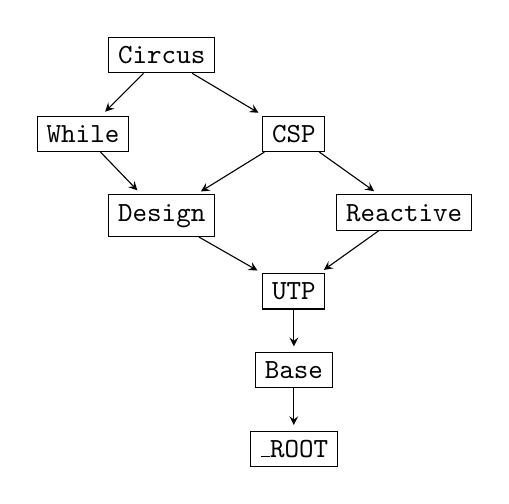
\begin{tikzpicture}[>=stealth,->,shorten >=2pt,looseness=.5,auto]
     \matrix[matrix of nodes,
             nodes={rectangle,draw,minimum size=4mm},
             column sep={1cm,between origins},
             row sep={1cm,between origins}]
      {              & |(X)|\texttt{Circus}  \\
        |(W)|\texttt{While} &              & |(C)|\texttt{CSP}                 \\
                     & |(D)|\texttt{Design} &              & |(R)|\texttt{Reactive}  \\
                     &              & |(u)|\texttt{UTP}              \\
                     &              & |(b)|\texttt{Base}                   \\
                     &              & |(r)|\texttt{\_ROOT}                 \\
      };
      \draw(X) -- (W) ; \draw (X) -- (C) ;
      \draw(W) -- (D) ; \draw (C) -- (D) ; \draw (C) -- (R) ;
      \draw (D) -- (u) ; \draw (R) -- (u) ;
      \draw (u) -- (b) ;
      \draw (b) -- (r) ;
    \end{tikzpicture}
  \caption{A Hierarchy of \texttt{Theory}s}
  \label{fig:hier-of-theory}
\end{figure}
Here we see theory slices organised as an acyclic directed graph,
where each slice inherits material from those below it.
At the bottom we have the \texttt{\_ROOT Theory} (slice),
which is hardwired in%
\footnote{
\texttt{\_ROOT} is the only thing hardwired---all other slices and their hierarchy
can be custom-built to suit the user.
}%
, and simply contains just the axioms of the underlying logic.

When we start a proof of a conjecture,
we do so from a given theory slice.
Imagine as an example, we state the following conjecture as part of theory \texttt{While}
(a simple imperative language):
\[
  \LNAME{$:=$-self-seq}
  \quad
  ( x:= e \comp x := f) =  x := f[e/x]
\]
We then start operating in a \emph{Proof Context} that consists
of the sequence of theory slices from \texttt{While} down to\texttt{ \_ROOT}.
This defines all the information about laws, definitions, know observation variables
that are in scope at the point were the conjecture is defined.
A successful proof of such a conjecture will result in it being added
to the collection of laws associated with its theory,
namely \texttt{While} in this example.

Another important principle is that when matching part of the proof of
{\LNAME{$:=$-self-seq}}
against a law in the \texttt{UTP} theory (say), the proof context is
shrunk to that from \texttt{UTP} down.
This is to ensure that specific uses of a name in a higher theory
(e.g. $J$ in Design, as per {\LNAME{$J$-def}})
does not mask a possible general use of $J$ as a schematic variable
in a lower theory%
\footnote{Variable $J$ may not be a plausible general predicate variable,
but $B$ is, and yet it is given a specific definition in \texttt{Reactive}.}%
.

\section{Logic}\label{sec:logic}

\PLAN{Describing the logic of \UTP2,
and why it isn't just plain old predicate calculus (first order).}

The logic of \UTP2\ is an adaptation of the first-order equational logic
described by Tourlakis \cite{journals/logcom/Tourlakis01},
that fully formalises the logic of Dijkstra, Gries and Schneider \cite{gries.93}.
\subsection{\UTP2\ Logic Syntax}

We define our logic syntax
over a collection of given sets characterising different name-spaces:
\RLEQNS{
   x,y,z \in Var && (given) & \mbox{Obs. Variables}
\\ k \in Const && (given) & \mbox{Constants}
\\ f,g,h \in Name && (given) & \mbox{(Function) Names}
\\ E,F,G \in EName && (given) & \mbox{Expression Metavariable Names}
\\ P,Q,R \in PName && (given) & \mbox{Predicate Metavariable Names}
}
Variables, constants and function names are as one would expect
in a logic with associated equational theories,
but we also have explicit meta-variables for expressions
and predicates, in the object logic, as many UTP laws
are expressed using such.

Expressions and Predicates are defined by mutual induction,
because both may contain instances of the other.
Expressions denote values in the ``world of discourse'' (observations)
and are typed. Expressions whose type is boolean ($c \in Expr$)
form the class
of \emph{atomic predicates}:
\RLEQNS{
   c,e \in Expr &::=& k | x  & \mbox{Expressions}
\\              &|& f~e & \mbox{Applications}
\\              &|& \lambda x @ e & \mbox{Obs. Abstraction}
\\              &|& \Lambda E @ e & \mbox{E-var. Abstraction}
\\              &|& \Lambda P @ e & \mbox{P-var. Abstraction}
\\              &|& \setof{ x | p @ e } & \mbox{Comprehension}
\\              &|& E & \mbox{Explicit Metavariable}
%\\              &|& e[ e/x ] & \mbox{Explicit Obs. Substitution}
%\\              &|& e[ e/E ] & \mbox{Explicit E-var. Substitution}
%\\              &|& e[ p/P ] & \mbox{Explicit P-var. Substitution}
}
Predicates are defined much as expected:
\RLEQNS{
   p,q,r \in Pred &::=& True | False & \mbox{Constant Predicates}
\\              &|& e & \mbox{Atomic Predicate (Boolean-valued Expr.)}
\\              &|& \lnot p & \mbox{Negation}
\\              &|& p~ \maltese q & \mbox{Composites, }\maltese \in \setof{\land,\lor,\implies,\equiv}
\\              &|& P & \mbox{Explicit Metavariable}
\\              &|& \yen x @ p & \mbox{1st-order Quantifiers, } \yen \in \setof{\forall,\exists,\exists!}
\\              &|& \yen P @ p & \mbox{higher-order Quantifiers, } \yen \in \setof{\mathbf\forall,\mathbf\exists}
\\              &|& \yen E @ p & \mbox{higher-order Quantifiers, } \yen \in \setof{\mathbf\forall,\mathbf\exists}
\\              &|& [ p ] & \mbox{Universal Closure (over observations)}
%\\              &|& p[ e/x ] & \mbox{Explicit Obs. Substitution}
%\\              &|& p[ e/E ] & \mbox{Explicit E-var. Substitution}
%\\              &|& p[ p/P ] & \mbox{Explicit P-var. Substitution}
}
%One point to note is that the syntax for both expressions
%and predicates include explicit substitutions,
%as these feature prominently in many UTP theories
%(e.g. laws regarding assignment and sequential composition,
%of the reactive healthiness condition \RR2).

The axioms of the logic are shown in Appendix \ref{sec:rules}
(\ref{ssec:prop-axioms}, \ref{ssec:non-prop-axioms}).
The axioms are stored in the hardwired \texttt{\_ROOT} theory,
in the \emph{laws} component of the theory,
which maps law-names to laws,
where a law is a predicate and a side-condition.
Side-conditions are a conjunction of zero or more basic conditions,
which typically capture relationships between given variables and
the free variables ($\fv$) of given predicates.
\begin{eqnarray*}
Theory &=& \textbf{record}
\\ && laws : Name \pfun Law
\\   && \ldots \textbf{end}
\\ Law &=& Pred \times Side
\\ Side &=&  x \notin \fv.P | \setof{x,y,\ldots} = \fv.P | \setof{x,y,\ldots} \supseteq \fv.P | \ldots
\end{eqnarray*}
Here the notation $A \pfun B$ denotes a partial finite function from $A$
to $B$, and so is effectively a table using a key of type $A$ to lookup
a value of type $B$.

The inference rules (\ref{ssec:inference})
are implemented, in the main, by a pattern matching mechanism
that takes a current proof goal and sees which laws can apply,
and a process that allows the user to select and apply the desired one,
storing the changed goal in a list that is assumed to be chained
together by logical equivalence.
The basic structural match has a judgement $\Gamma\vdash P \ddagger T | \beta$
that asserts that,
given matching environment $\Gamma$,
test predicate $T$ matches pattern predicate $P$, with resulting bindings $\beta$.
Bindings map variables to well-formed expressions or predicates,
as appropriate.
If we ignore $\Gamma$ for now, then a representative collection
of structural matching rules are:
\begin{eqnarray*}
   & \inferrule%
      {}%
      {\Gamma \vdash x \ddagger e |\setof{ x \mapsto e} }
   & \LNAME{match-var}
\\
\\ & \inferrule%
     {\Gamma\vdash P_i \ddagger T_i  | \beta_i
       \qquad
       \beta_1 \cong \beta_2}%
     {\Gamma \vdash P_1 \land P_2 \ddagger T_1 \land T_2 | \beta_1 \uplus \beta_2}
   & \LNAME{match-$\land$}
\\
\\ & \inferrule%
        {P \ddagger Q  | \beta_1
          \qquad xs \ddagger ys | \beta_2
          \qquad \beta_1 \cong \beta_2}%
        {\forall xs @ P \ddagger \forall ys @ P | \beta_1 \uplus \beta_2}
   & \LNAME{match-$\forall$}
\end{eqnarray*}
The $\cong$ predicate asserts that two bindings
do not map the same variable to different things.
The $\uplus$ operator merges two bindings, provided they satisfy $\cong$.
An attempted match of $T$ against $P$ fails if no rules apply,
or an attempt is made to apply $\uplus$ to two bindings that do not satisfy $\cong$.

In order to facilitate proof, the theory has two components, one
for conjectures, which can be viewed as aspirant laws
(posited, hopefully true, but not yet proven),
and theorems, which are conjectures with proofs:
\begin{eqnarray*}
Theory &=& \textbf{record} \ldots
\\ && conjs : Name \pfun Law
\\ && thms : Name \pfun Proof
\\ && \ldots \textbf{end}
\\ Proof &=& \textbf{record}
\\ && goal : Pred
\\ && sc : Side
\\ && done : \Bool
\\ && \ldots \textbf{end}
\end{eqnarray*}
The workflow is as follows: conjectures can be entered by the user
and accumulated in $conjs$. A proof can then be started by selecting
a conjecture, which creates a corresponding entry in $thms$,
with $goal,sc$ set to match the conjectured law, and the $done$ flag
set to false. More than one proof can be active at any one time.
A proof is carried out using all the $laws$ accessible from
the theory.
Once a proof is complete, the $done$ flag is set true,
the corresponding conjecture is deleted, and, usually,
a corresponding entry is made into $laws$.

The mechanism as described so far is adequate for proving all and any conjectures
based on propositional logic.
However it needs extensions to cater for non-propositional logic,
and the datatype theories.
We will address the non-propositional extensions in the next section
on generic UTP.
Here we discuss briefly some practical issues with datatype theories.
We can define a theory of natural number arithmetic using Peano axioms,
for example---the tool supports the creation of a new named empty
theory, and the addition of appropriate axioms%
%\footnote{
%Exercise: you need five axioms --- what are they?
%}
 by the user into the $laws$ table.
Operations on natural numbers can be defined axiomatically by adding further
laws as required.
From this it is possible to prove a range of theorems about natural number
operations, e.g. $m + 0 = m$.
A similar exercise can be done for sets, and sequences,
resulting in laws like $S \cup \emptyset = S$ and $s \cat \nil = s$.
The problem is that we do not just match against whole laws, but can also
match against just the lefthand or righthand sides of an equality or
equivalence---so the righthand sides of all three laws above will match
an arbitrary expression $e$, offering $e+0$, $e \cup \emptyset$ and $e \cat \nil$
as replacements.
To prevent such spurious matches, we introduce a type system for expressions,
and a type-inference engine, that uses context information to deduce the types
of expressions like $e$, and serves to reduce spurious matches to a considerable degree.
A theory contains tables to support this feature:
\begin{eqnarray*}
Theory &=& \textbf{record} \ldots
\\ && type : Name \pfun Type
\\ && \ldots \textbf{end}
\\ t \in Type &::=& \Bool | \Int | \tau | \power t | \ldots
\end{eqnarray*}
The $Name$s in $type$ are typically names of variables or functions.

\section{UTP}\label{sec:utp}

\PLAN{ Describing the more ubiquitous operators of UTP,
and why we want to handle alphabets implicitly.}

Some key concepts are common to most UTP theories,
namely sequential composition ($\comp$), non-deterministic choice ($\sqcap$),
refinement ($\refinedby$) and conditional ($\cond c$).
Importantly, in most theories these all have the same definition:
\begin{eqnarray*}
% \nonumber to remove numbering (before each equation)
  P \comp Q &\defs& \exists Obs_m @ P[Obs_m/Obs'] \land Q[Obs_m/Obs] \\
  P \sqcap Q &\defs& P \lor Q \\
  P \refinedby Q &\defs& [ Q \implies P ] \\
  P \cond c Q &\defs& c \land P \lor \lnot c \land Q
\end{eqnarray*}
The definitions for $\sqcap$, $\refinedby$ and $\cond c$ are unproblematical,
and are easily handled by the existing machinery,
with one key extension.
The definition of $\comp$ not only makes use of explicit substitution notation,
but also raises the question of how to interpret $Obs_m$, $Obs'$ and $Obs$.
Clearly they stand for the obervational variables of a UTP theory along with
appropriate decorations, but how do we support this?
In particular, how can we arrange matters so that
we only define $\comp$ once, in such a way that it can be used by many different theories?
We will first address the key extension alluded to above,
and then return to the problem of sequential composition.

\subsection{Defining your own language in \UTP2}

A key aspect of a UTP theory is the signature that captures the
abstract syntax of the language being defined.
This means that \UTP2\ needs to support user-defined languages.
This is achieved by having a table-driven parser for entering predicates,
and providing a facility for the user to add new entries
to the relevant tables:
\begin{eqnarray*}
Theory &=& \textbf{record} \ldots
\\ && precs : Name \pfun Precedence
\\ && lang : Name \pfun LangSpec
\\ && \ldots \textbf{end}
\end{eqnarray*}
The $precs$ table maps the name of an infix operator
to information about its parsing precedence and its associativity.
The $lang$ table maps a language construct name to a language specification
($LangSpec$) that describes the concrete syntactical structure of that construct.
A language specification is a mix of keywords denoting syntactical components
like variables (V) , expressions (E) , predicates (P),
 or various lists of such,
interspersed with concrete syntax symbols.
We won't give a full definition here but present some examples to give the
idea:
\begin{itemize}
  \item
    Refinement: we specify this as ``\verb@P |= P@'',
  which states that \verb@|=@ is an infix operator between two predicates.
  When this is entered into the $lang$ table,
  a corresponding entry is automatically created in the $precs$
  table with default values (mid-range precedence, non-associative)
  which can then be edited by the user to suit.
  Also entered is a dummy definition for the construct
  into the $laws$ table, which itself then needs to be edited.
  \item Assignment:
    specified as ``\verb@V := E@'', stating that \verb@:=@
    is an infix operator in-between a variable and expression,
    resulting in a predicate.
\end{itemize}
In general defining a language construct (resulting in a predicate)
 involves adding entries
to the $lang$ and $laws$ tables,
and possibly also to the $types$ and $precs$ tables, depending
on the precise nature of the construct.
Infix expression operators do not have $lang$ entries
but require $laws$, $precs$ and $types$ entries.

When we talk about developing a theory of Designs (Section \ref{sec:designs}),
we shall give a worked-out example of  a language definition.

\subsection{The problem with $\protect\comp$}

The definition of sequential composition,
\begin{eqnarray*}
P \comp Q &\defs& \exists Obs_m @ P[Obs_m/Obs'] \land Q[Obs_m/Obs]
\end{eqnarray*}
says in effect that for each observation, $x$, say, in $Obs$,
we replace any free occurrence of $x'$ in $p$ by $x_m$
and any free occurrence of $x$ in $q$ by $Obs_m$,
and use existential quantification to hide $x_m$.
In effect the rule above is really a rule-schema,
characterising an infinite number of rules,
one for each possible alphabet represented by $Obs$.
However, we don't want to repeatedly instantiate this rule
and reason about its consequences for each specific alphabet we use.
In fact, we want to use the definition in cases where only part
of the alphabet is known (Designs again, Section \ref{sec:designs}).
We would prefer to be able to do proofs with the definition
as given above, only instantiating $Obs$ where necessary,
and then perhaps only partially.
In fact, we want to support the following proof
(of the associativity of $\comp$)
which does not require any instantation of $Obs$:
{\small
\begin{eqnarray*}
  && P ; (Q ; R)
\\&\equiv& \exists Obs_m @ P[Obs_m/Obs']
           \land (Q;R)[Obs_m/Obs]
\\&\equiv& \exists Obs_m @ P[Obs_m/Obs']
           \land (\exists Obs_n @ Q[Obs_n/Obs'] \land R[Obs_n/Obs])[Obs_m/Obs]
\\&\equiv& \exists Obs_m,Obs_n @ P[Obs_m/Obs']
           \land Q[Obs_n/Obs'][Obs_m/Obs]
           \land R[Obs_n/Obs][Obs_m/Obs]
\\&\equiv& \exists Obs_m,Obs_n @
                  P[Obs_m/Obs'][Obs_n/Obs']
           \land Q[Obs_n,Obs_m/Obs',Obs]
           \land R[Obs_n/Obs]
\\&\equiv& \exists Obs_n @
                  (\exists Obs_m @ P[Obs_m/Obs'][Obs_n/Obs']
           \land Q[Obs_m/Obs][Obs_n/Obs'])
\\&& \qquad\qquad {} \land R[Obs_n/Obs]
\\&\equiv& \exists Obs_n @
                  (\exists Obs_m @ P[Obs_m/Obs']
           \land Q[Obs_m/Obs])[Obs_n/Obs']
           \land R[Obs_n/Obs]
\\&\equiv& \exists Obs_n @
                  (P ; Q)[Obs_n/Obs']
           \land R[Obs_n/Obs]
\\&\equiv&(P ; Q) ; R
\end{eqnarray*}
}
In effect we want to reason within our logic about ``schematic''
variables like $Obs$ and treat the substitution notation as part
of the object logic, rather than meta-notation describing
the behaviour of an inference rule.

To achieve this we have to add another linguistic innovation
to the logic.
A common shorthand in most presentations of logic is to
view $\forall x,y,z @ p$ (say)
as a shorthand for $\forall x @ \forall y @ \forall z @ p$.
Our innovation is not only to add the former as a full part
of the logic syntax, but also a further extension.
We want to be able to have quantifier variables (e.g. $Obs$)
that represent lists of ``ordinary'' quantifier variables.
We do this by splitting the list into two parts, separated by
a semi-colon, with those in the first part being ordinary,
whilst those in the second part denote lists of variables.
The revised syntax of $\forall$ is now:
$$
\forall x_1,\ldots,x_m \qsep xs_1, \ldots , xs_m @P
\qquad
m \geq 0, n \geq 0, m+n \geq 1
$$
Other observation (1st-order) quantifiers are modified similarly.
The $x_i$ and $xs_j$ above are ``quantifier variables'',
and will be disambiguated were necessary by referring to the $x_i$
(before the $\qsep$ sysmbol) as ``single variables''
and the $xs_j$ (after $\qsep$ as ``list variables'').
A list where $m=0$ is referred to as an ``ordinary list''.
The meaning of a quantifier variable list of the
form $x_1,\ldots,x_m \qsep xs_1, \ldots , xs_m$
is that it matches an ordinary list
of the form $y_1,\ldots,y_{m+k}, k \geq 0$
where each $x_i$ binds to one $y_j$,
each $xs_i$ binds to zero or more $y_j$,
and every $y_j$ is bound exactly once.
In principle the bindings associated with a variable like $xs_i$
are non-deterministic, albeit they must be consistent with bindings derived
from the match as a whole, i.e. the wider context in which that  variable occurs.
In practice, heuristics are used in the implementation to select
a binding that is hopefully as ``good'' as possible.

As our proof above largely depended on properties of (explicit)
substitution, we have to add it into our logic as well.
So we revise our syntax for predicates:
\RLEQNS{
   p,q,r \in Pred &::=& \ldots
\\              &|& \yen qvs @ p & \mbox{1st-order Quantifiers, } \yen \in \setof{\forall,\exists,\exists!}
\\              &|& p[ e/x ] & \mbox{Explicit Obs. Substitution}
\\              &|& p[ e/E ] & \mbox{Explicit E-var. Substitution}
\\              &|& p[ p/P ] & \mbox{Explicit P-var. Substitution}
\\ qvs \in QVars &&& \mbox{Quantifier Variable lists}
\\ &::=~& x_1,\ldots,x_m \qsep xs_1, \ldots , xs_m
   & m \geq 0, n \geq 0, m+n \geq 1
}
Explicit substitutions are also added to expressions as well.
Laws regarding explicit substitutions also need to be developed,
e.g.
$$
p[e/x][f/y] = p[e,f/x,y], \quad x \neq y, y \notin \fv.e
$$
but we do not list these here.

This extension allows us to introduce axioms like:
$$
\AXallOInst \qquad \AXallOInstN
$$
rather than relying on a simple single quantifier axiom
and the usual conventions regarding the $\forall x,y,z$ shorthand.
In essence what we have done is to formalise and automate this convention.

To support the definition of $\comp$ we need one further step.
The list variable $Obs$ does not stand for an arbitrary
list of single variables, but is instead intended to stand for
precisely those un-dashed variables that are present in the
alphabet of the current theory, even if that alphabet
has not been fully described.
Similarly, $Obs'$ stands for all the dashed variables,
and $Obs_m$ denotes the decoration of all the $Obs$ variables.
In effect we designate certain list variables (like $Obs$)
as having a special meaning.

The basic matcher described in Section \ref{sec:logic},
has to be enhanced to perform appropriate matching
where non-ordinary quantifier lists are present.
To make this work, we need to extend theories to have
a table that records the theory alphabet:
\begin{eqnarray*}
Theory &=& \textbf{record} \ldots
\\ && obs : Name \pfun Type
\\ && \ldots \textbf{end}
\end{eqnarray*}
The $obs$ table needs to become part of the matching context $\Gamma$,
and we introduce rules for matching quantifier lists:
\begin{eqnarray*}
  & \inferrule%
       {~}%
       {\Gamma \vdash \qsep Obs \ddagger \qsep Obs | \varepsilon }
\\
\\& \inferrule%
       {Obs(\Gamma)=\setof{o_1,\ldots,o_n}}%
       {\Gamma \vdash \qsep Obs \ddagger \setof{o_1,\ldots,o_n}
         | \setof{Obs \mapsto \setof{o_1,\ldots,o_n}}}
\end{eqnarray*}
The first rule allows $Obs$ to match itself, and so we can do proofs
that do not require it to be expanded to an ordinary list.
Note also that in this case an empty binding ($\varepsilon$) is returned.
Other matching rules not shown here, take care of decorations,
ensuring that $Obs$ matches $x,y,z$, if appropriate,
but not $x',y',z'$.

We can now define sequential composition in our revised logic as:
\begin{eqnarray*}
P \comp Q &\defs& \exists \qsep Obs_m @ P[Obs_m/Obs'] \land Q[Obs_m/Obs]
\end{eqnarray*}
and produce a proof as shown earlier.
There is an additional extension required to the logic to do this,
but we shall motivate and introduce it
in the section on Designs (Section \ref{sec:designs}).

\section{Designs}\label{sec:designs}

\PLAN{A theory of designs is developed, showing implicit and explicit alphabets,
and the importance of side conditions.}

The UTP theory of Designs \cite[Chp 3]{UTP-book}
introduces two boolean observation variables ($ok, ok'$)
to model program start and termination, and new notation $P \design Q$
to represent a predicate with pre and post-conditions:
\begin{eqnarray*}
  ok,ok' &:& \Bool \\
  P \design Q &\defs& ok \land P \implies ok' \land Q
  , \qquad ok,ok' \notin \fv.P \cup \fv.Q
\end{eqnarray*}
A key feature to note is that in this theory we do not specify
the entire alphabet, but only stipulate that whatever it is,
it must contain $ok$ and $ok'$.
In this light we see an even stronger need for special list-variables
like $Obs$ as already introduced.

We can already capture this with our theories as described so far:
\begin{eqnarray*}
   obs(ok) &=& \Bool
\\ obs(ok') &=& \Bool
\\ lang(\design) &=& P \design P
\\ prec(\design) &=& (n,NonAssoc), \quad n \mbox{ is desired precedence}
\\ laws(\design\!-\!DEF)
   &=& (P \design Q \equiv ok \land P \implies ok' \land Q,
        ok,ok' \notin \fv.P \cup \fv.Q)
\end{eqnarray*}
Here we see some side-conditions that assert that neither $P$ nor $Q$ should
mention either $ok$ or $ok'$.
These are important side-conditions, without which we do not obtain the
desired behaviours (algebraic laws) for designs.
However, in proving properties of designs in UTP,
we find that the side-conditions play a more active role than encountered
in more traditional presentations of logic.
In many logics, side-conditions about free variables
are syntactic in nature and can always be checked/discharged
when applying a rule to a predicate in the logic.
In particular, when applying a rule like the one above, both $P$ and $Q$
will have been instantiated to concrete predicates, and so it will be
easy to establish the truthfulness of these side-conditions.
However in a UTP proof about the properties of designs,
we work with explicit meta-variables $P$ and $Q$
for which it is not possible to compute side-condition rules
at rule-application time.

Instead, we have to add a post processing stage to law matching.
Assuming that a target predicate match involving a law has succeeded
returning a binding,
We use that binding to translate any side-condition with the law
to a corresponding one in the target world.
We then need to show that the translated law-side condition
is a consequence of any side-conditions associated with the conjecture goal.

In effect, in addition to a syntax for side-conditions,
we have to implement a side-condition inference engine
that can deduce when one side-condition implies another.
Let $psc$ denote the translated pattern side-condition,
and $tsc$ denote the side-condition associated with the conjecture being proven.
We have to demonstrate that $tsc \implies psc$.
As side-conditions are a conjunction of a few basic primitive side-conditions,
we simply take both $tsc$ and $tsc \land psc$,
reduce both to a canonical normal form, and check for equality.


To illustrate all of this, here is a proof that $R \design S \equiv R \design R \land S$,
given that $ok, ok' \notin \fv.R \cup \fv.S$.
Here we deliberately state our conjecture using different meta-variables
to those used to define designs, to show the translation aspect at work.
Our proof strategy will be to take the lefthand side
and transform it into the righthand side%
\footnote{
The strategy in play is noted in the $Proof$ record.
}%
.

The first step  proceeds when a match of $R \design S$ succeeds
against pattern $P \design Q$ returning the binding $\mapof{P \mapsto R, Q \mapsto S}$.
However, we need to discharge the side-condition $ok,ok' \notin \fv.P \cup \fv.Q$.
We use the bindings to translate this to $ok,ok' \notin \fv.R \cup \fv.S$.
This then has to be implied by our conjecture side-condition, which in this case
is identical to the law condition, so
we can deduce that it holds.
The proof then proceeds as follows:
\begin{eqnarray*}
  && R \design S
\EQV{as just discussed above}
\\&& ok \land R \implies ok' \land S
\\&\quad\equiv\quad& ok \implies ( R \implies ok' \land S)
\\&\equiv& ok \implies ( R \implies R \land ok' \land S)
\\&\equiv& ok \land R \implies ok' \land S \land R
\EQV{see below}
\\ && R \design R \land S
\end{eqnarray*}
The last step up is similar to the first, as the matching of righthand sides
succeeds, and the bindings and translation are the same.
This raises a new and important issue to do with observational variables.
The variables $ok$ and $ok'$ mentioned above are not arbitrary,
but denote specific observations, and so it is important for UTP that
they only match themselves in laws, unlike general variables
that can match arbitrary expressions (including other variables).
This leads to the need to indicate that certain variables in patterns
stand for themselves. Such variables are described as being ``known''.
All $obs$ variables are known,
and there is also a facility for a user to give names to constants and expressions,
and so those names would also be considered ``known''.
We will not give further details here.

The structural matching rule for variable patterns needs to be modified,
using the context $\Gamma$ to check if a variable is known,
here written as $x \in \Gamma$:
\begin{eqnarray*}
  & \inferrule%
       {x \in \Gamma}%
       {\Gamma \vdash x \ddagger x }
\\& \inferrule%
      {x \notin \Gamma}%
      {\Gamma \vdash x \ddagger v |\setof{ x \mapsto v} }
\\& \inferrule%
      {x \notin \Gamma}%
      {\Gamma \vdash x \ddagger e |\setof{ x \mapsto e} }
\end{eqnarray*}
Note that when a known variable matches against itself, no binding entry
is produced.

At this point, given the hierarchy of Figure \ref{fig:hier-of-theory},
we have a theory called \texttt{Design},
which has access to the laws of logic, equality, arithmetic and sets,
as well as the definitions and associated laws of $\comp$, $\sqcap$, $\refinedby$,
$\cond c$ and $\design$, as well as the known observation variables $ok$ and $ok'$.
In particular, we stress that by being linked in the hierarchy shown,
the \texttt{Design} theory inherits all the material defined in \texttt{UTP}, and all its
ancestors.
This is quite abstract at this point, so now we move to ground it all a little more.

\subsection{Healthiness Conditions}

A key feature of UTP is the use of healthiness conditions,
expressed typically as monotonic idempotent predicate transformers.
To support this in \UTP2\, we need to extend the predicate syntax
to include notation for functions over predicates, and the application
of those to predicates, and appropriate axiomatisation:
\begin{eqnarray*}
   p,q,r \in Pred &::=& \ldots
\\              &|& \Lambda P @ p, \qquad  \mbox{Predicate Abstraction}
\\              &|& p(q), \qquad \mbox{Predicate Application}
\\ (\Lambda P @ p)(r) &\equiv& p[r/P]
\end{eqnarray*}
It is at this point that we definitely leave 1st-order logic behind
and move up towards 2nd- and higher-orders of logic.
At this point it is useful to have a facility to give names
to frequently used constructs like  healthiness conditions
or common predicate fragments, such as the predicates called $II$, $B$ and $J$
used in the definition of the Reactive theory \cite[Chp. 8]{UTP-book}.
In effect we want to give definitions like the following
(not necessarily from the theory of Designs):
\begin{eqnarray*}
   \H1 &\defs& \Lambda P @ ok \implies P
\\ J &\defs& (ok \implies ok') \land wait=wait \land tr'=tr \land ref'=ref
\end{eqnarray*}
We achieve this by adding in tables into a theory that allow us
to write such definitions,
and modifying the matching algorithm to treat all names in those
tables as ``known'':
\begin{eqnarray*}
Theory &=& \textbf{record} \ldots
\\ && preds : Name \pfun Pred
\\ && exprs : Name \pfun Expr
\\ && \ldots \textbf{end}
\end{eqnarray*}
So, for example,
in this theory of Designs we have $preds(\H1) = \Lambda P @ ok \implies P$.
The rest of the \UTP2\ machinery can then be used to reason about and use these
healthiness conditions in the normal way,
so for example, $\H1(q)$ can be converted into $ok \implies q$, and vice-versa.

\section{Programs}\label{sec:programs}

\PLAN{We now use Designs to develop a simple imperative language,
where our need to handle explicit substitutions becomes even more apparent.}

To get concrete, we are now going to define the semantics
for a simple imperative programming language (a.k.a. $While$),
as a UTP Design.
To keep things simple for now,
we assume the language has exactly three program variables:
 \texttt{x}, \texttt{y}, and \texttt{z}
(we look at the issue of many variables below in Section \ref{ssec:skip-n-assign}).
\RLEQNS{
   u,w \in While &::=& Skip & \mbox{do nothing}
\\              &|& v:=e & \mbox{Assignment, } v \in  \setof{x,y,z}, \fv.e \subseteq \setof{x,y,z}
\\              &|& u \comp w & \mbox{Sequential Composition}
\\              &|& u \cond c w & \mbox{Conditional, } \fv.c \subseteq \setof{x,y,z}
\\              &|& c \circledast w & \mbox{While-loop, } \fv.c \subseteq \setof{x,y,z}
}
The alphabet of this theory now contains $x,y,z,x',y',z'$
in addition to $ok,ok'$ inherited from the Design theory.
Also inherited are the definitions of $\comp$ and $\cond c$,
where now $Obs$ can bind to $ok,x,y,z,ok',x',y',z'$
in pattern matching.
We can use the language specification facility to introduce the syntax
to \UTP2, so in $While.lang$ we have:
\begin{eqnarray*}
   Skip & \mapsto & \texttt{Skip}
\\ :=  & \mapsto & \texttt{V := E}
\\ whl & \mapsto & \texttt{E ** P}
\end{eqnarray*}

\subsection{The \UTP2\ semantics of $Skip$ and $x:=e$}
\label{ssec:skip-n-assign}

We start to define the semantics of $Skip$,
and we could immediately write:
\begin{eqnarray*}
  Skip &\defs& True \design x'=x \land y'=y \land z'=z
\end{eqnarray*}
While correct, we may worry about what happens if the number of variables
increases, or if we want to have some dynamism regarding the number and
names of program variables. While we discuss another possible approach
to program variables later, for now let's see what we can do to improve things.
We could try to use special list variable $Obs$,
to get
\begin{eqnarray*}
  Skip &\defs?& True \design Obs' = Obs
\end{eqnarray*}
but this is not satisfactory, as $Obs$ ($Obs'$) includes $ok$ ($ok'$)
and these cannot occur in the design predicates, as per the side-condition
used in the Design theory.

The solution here is realise that in many UTP theories
we actually have two classes of observations: those associated with
the values of variables in the program text under consideration (here $x$, $y$ and $z$),
and those that capture overall program properties, independent of any program variable
(here $ok$ and $ok'$, denoting termination).
We shall refer to the former as script variables and the latter as model variables,
and add in two new special list-variables called $Scr$ and $Mdl$
to match against the two classes.
So in this theory, $Scr$ can match $x,y,z$, while $Mdl$ matches $ok$.
Also $Obs$ can now match $Scr,Mdl$, or combinations such as $Scr,ok$.
This requires us to modify the $obs$ table in a theory slightly
as we must now record observation class, as well as its type:
\begin{eqnarray*}
Theory &=& \textbf{record} \ldots
\\ && obs : Name \pfun Type \times OClass
\\ && \ldots \textbf{end}
\\ OClass &::=& Model | Script
\end{eqnarray*}
So, for example, in theory \texttt{Design} we have $obs(ok) = (\Bool,Model)$,
while in theory \texttt{While} we have $obs(x) = (t,Script)$, where $t$ is some type.
We can now define the semantics of $Skip$ as:
\begin{eqnarray*}
  Skip &\defs& True \design Scr'=Scr
\end{eqnarray*}
This definition will now work in a range of theories,
provided the observations are classified appropriately.
However it does also require a further extension
of the law matching algorithm.
This has to be modified to allow a pattern like $Scr'=Scr$,
given bindings $Scr \mapsto x,y,z$ and $Scr' \mapsto x',y',z'$,
to match against a predicate fragment like $x'=x \land y'=y \land z'=z$.
This feature is quite easily implemented as part of the structural matcher.

We now turn our attention to the definition of assignment.
The following is \emph{not} satisfactory:
\begin{eqnarray*}
  x:=e &\defs?& True \design x' = e \land Scr'=Scr
\end{eqnarray*}
First, as $x$ is known, this rule will only match assignments whose
variable is $x$, so we would need a different definition for each program
variable---not a good idea!
Secondly, $Scr'=Scr$ will match $x'=x \land y'=y \land z'=z$
as already described, and so we can match $x'=e \land x'=x$
which reduces to $x=e$, and then probably $False$.
We could try to make the matching of $Scr'=Scr$ against
$x'=x \land y'=y \land z'=z$ ``context sensitive'',
only matching an equality if both sides do not appear ``elsewhere'',
but it is currently very unclear if this is at all feasible.
Instead, we extend the list-variable notation to allow modifiers,
so we can write the following satisfactory definition for assignment:
\begin{eqnarray*}
  v:=e &\defs& True \design v' = e \land (Scr'\setminus v')=(Scr\setminus v)
\end{eqnarray*}
The law/pattern variable $v$ is not known, so it will match any of $x$, $y$ or $z$,
and even $ok$.
However as $ok$ cannot appear in the predicates in a design,
any matching of $v$ to $ok$ will lead to a proof that eventually freezes
up because the side-condition defining $\design$ won't be satisfiable.
Imagine we are matching the righthand side of the above definition
with $y'=f \land x'=x \land z'=z$.
The matching algorithm will attempt match $y'$ against $v'$,
returning a binding $v' \mapsto y'$.
This binding gives us enough information
to be able to match
$(Scr'\setminus v')=(Scr\setminus v)$
against $x'=x \land z'=z$.

A further complication arises when we try to prove laws such
as:
\begin{eqnarray*}
   (v:=e \comp v:=f ) &\equiv&( v := f[e/v])
\\ (u:=e \comp v:=f) &\equiv& (v := f[e/u] \comp u := e),
    \quad v \notin \fv.e
\end{eqnarray*}
We will not elaborate on details here,
but we find the need to use special list variables like $Scr$ and $Scr'$
in substitutions, so the matching algorithm needs to handle those cases as well.

\subsection{Merging program variables}

Another way to handle program variables
is to group them together into an environment,
a mapping from variable names to values:
\begin{eqnarray*}
% \nonumber to remove numbering (before each equation)
  \rho \in Env &=& Var \pfun Val
\end{eqnarray*}
We can then introduce $Model$ variables
called $state$ and $state'$.
This simplifies the alphabet handling, as it is now fixed,
and we can model variable declarations with map extensions.
In effect we have no script variables, just model ones,
with the consequence that the theory of the alphabet is now
independent of the program script.
The added complexity now emerges in the type system,
because $Val$ needs to include all types in $Type$,
and the definition of assignment now requires an $eval$
function of type $Env \fun Expr \pfun Val$
(here $\oplus$ denotes map override):
\begin{eqnarray*}
  v:=e &\defs& True \design state'=state \oplus \setof{v \mapsto eval(state)(e)}
\end{eqnarray*}
\UTP2\ can support either style of program variable handling,
although the environment-based approach requires a theory
of finite maps, and laws defining $eval$ for every expression construct,
with an added complication of having to handle explicit expression \emph{syntax} in laws.
However, the provision of such an $eval$ function is not quite as onerous as it sounds
as laws providing the meaning of all expression constructs
are required in any case.


%\subsection{The \UTP2\ semantics of $c \circledast w$}

We are not going to elaborate too much on how to give
a semantics to the while-loop construct here,
apart from noting that it requires a fixpoint construct
in the logic syntax, and an appropriate axiomatisation of fixpoint theory.
Then the loop can be defined as the least fixed point of
the appropriate functional.
\begin{eqnarray*}
   p,q,r \in Pred &::=& \ldots
\\              &|& \mu P @ F(P) \qquad \mbox{Fixpoint Operator}
\\ c \circledast w &\defs& \mu W @ (w \comp W) \cond c Skip
\end{eqnarray*}

\section{Soundness}\label{sec:soundness}

\PLAN{What basis does anyone have for trusting the output of \UTP2?}

Is \UTP2\ sound?
For now, the simple answer is no,
due mainly to two reasons.

Firstly, users can add their own laws (axioms),
and this always leads to the risk of defining a theory that is inconsistent.
As we consider the typical user to be a UTP practitioner with experience in logic
and axiomatics, developing foundational theories,
we feel it is reasonable to expect such (power) users
to be able to use their judgement to avoid such pitfalls.
Having said that, it will probably make sense in future versions
of the tool to support users at different levels of experience,
with the more advanced and dangerous features disabled for novices.

Secondly, the underlying proof engine is very complex,
reflecting the complexity of the logic required.
At present we are not in a position to guarantee soundness of every action
that can be invoked. However, in mitigation, we do point out that
the outcome of each basic proof step is highly visible in the tool's GUI.
It is clear that eventually we will have to pay serious attention
to ensuring the prover is sound (modulo any inconsistencies introduced
via user-defined axioms). We envisage two possible approaches:
\begin{enumerate}
  \item
    Identifying a very small core from which the whole logic can be developed
    conservatively, and producing a small piece of prover kernel code
    that can then be verified. This is the LCF approach adopted for prover systems
    like HOL\cite{books/sp/NipkowPW02} and Coq\cite{tr:Coq:manual:08}.
  \item
    Developing an encoding of the \UTP2\ logic into the logic of a system
    with a verified kernel, such as HOL or CoQ, and using those systems
    to do automated proof checks, possibly even for each proof step as it is
    done.
\end{enumerate}

\section{Exploitation}\label{sec:exploitation}

\PLAN{Having a nice UTP theory of something gives intellectual satisfaction,
but how do we turn it into something useful?}

Assuming that we have addressed the soundness of the implementation of \UTP2,
and have used it to develop a nice theory of an interesting language,
how useful will the results be if we try to apply them to a real problem?
In principle, we could use \UTP2\ to prove properties of a program
written in the language described by our theory.
In fact some work has already been done exploring
a feature that allows us to take a predicate-transformer theory
(e.g. weakest precondition, as per \cite[Chp. 2, p66]{UTP-book}),
and a program,
and automatically generate proof obligations.
However, \UTP2\ is an interactive proof assistant, designed
to support UTP theory development, rather than theory use.
In practise, there is no way that \UTP2\ can realistically compete
with existing industrial-strength tools that can both generate
and discharge such proof obligations with a high degree of efficiency.

However what does seem to be feasible, is to develop a facility
whereby a UTP theory, once complete,
can be translated and exported as a theory useable by just such industrial-strength
provers. We are currently exploring building such a theorem-prover link
to
HOL, as recent work has looked at encoding UTP
in ProofPower/HOL\cite{conf/utp/OliveiraCW06,conf/utp/ZC08},
or Isabelle/HOL \cite{conf/utp/FeliachiGW10,conf/vstte/FeliachiGW12}.
We hope to be able to make use of these results
to build such a \UTP2-to-HOL bridge.

\section{Conclusions}\label{sec:conclusions}

\PLAN{Wrap-up the paper.}

We can, in effect,
summarise the paper
 by giving a requirements list summarising all the special logic features we desire
 for \UTP2:
predicate and expression meta-variables;
user language definitions;
quantifier list variables, with specials to identify alphabets;
explicit substitutions;
``semantic'' side-conditions;
and
predicate transformers.

All the above could be implemented using Isabelle, or CoQ,
or PVS, or pretty much any higher-order theorem prover.
However any algorithm can, in principle, be written in the pure lambda
calculus, or expressed as a Turing machine,
but this does not make it
feasible, desirable or practical to use those notations.
Similarly we feel that encoding our requirements into one of the above higher-order
systems, at least to the extent that it would be visible to the user,
is not the way to meet our requirement for machine-assisted support
for UTP foundational reasoning.

The resulting logic is quite large, and space limitations have prevented
us from giving a complete description here.
More details can be found in a draft of the \UTP2\ Reference Manual
\cite{UTP2:Reference}.


\bibliography{SAOITHIN}

\appendix
\section{Rules}\label{sec:rules}

\PLAN{We present the current versions of axioms and inference rules.}

\subsection{Propositional Axioms}\label{ssec:prop-axioms}
$$
\AXPROP
$$
\subsection{Inference Rules}\label{ssec:inference}
$$
\INFERENCES
$$

\subsection{Non-propositional Axioms}\label{ssec:non-prop-axioms}
$$
\AXNONPROP
$$



%\subsection{Derived Rules}\label{ssec:derived}
%$$
%\DERIVED
%$$
%
%\subsection{Deduction}\label{ssec:deduction}
%$$
%\DEDUCTION
%$$
%
%\subsection{Matching}\label{ssec:matching}
%
%\subsubsection{Structural}\label{sssec:matching-struct}
%
We present here the basic structural matching rules

\MRSTRUCT

We have two versions of null-quantifier matching:
\begin{description}
  \item[\MRNullQuantZN] allows all list-variables in a quantifier
   to match empty lists,
   which results in a law like
   \[(\exists \lst x @ P) = \lnot(\forall \lst x @ \lnot P)\]
   being able to match
   \[ P = \lnot\lnot P, \qquad \textrm{with } \lst x \mapsto \nil \]
  \item[\MRNullQuantON] requires at least one list-variable in a quantifer
   to match a non-empty list, so preventing the above match.
\end{description}
Currently we adopt \MRNullQuantZN, with surprising (but so far, sound) results.
Using \MRNullQuantON\ might be preferable to avoid confusion though.
This should probably be something that can be toggled.

%
%\subsubsection{Known}\label{sssec:matching-known}
%Matching needs more than just the pattern and test:
it also requires a matching context ($\Gamma$)
that supplies information about various variables in order to
determine how they match.
The basic idea is that a pattern variable $v$ matches any corresponding
object, unless that variable is ``known'' ($v \in \Gamma$).
If a variable is known, then what it matches is governed
by what is known about it ($\Gamma(v)$).

It should be remembered that a pattern variable that is known
may occur in a pattern underneath a quantifier binding that variable,
in which case that instance of the variable is not known,
and is free to match any corresponding object.
A pattern variable in a quantifier binding list 
is not ``known'', but is restricted to matching only other
binding list variables.

\subsubsection{Known Names}

We supply as a context the following trie lists:
\begin{itemize}
  \item observation variables
  \item type variables denoting types
  \item variables denoting constants
  \item e-variables denoting expressions
  \item p-variables denoting predicates
\end{itemize}
the first being observation variables,
whilst the rest are the known (named) 
types/variables/expressions/predicates in each context.
A pattern variable not listed as known, matches anything of the corresponding type:
\begin{itemize}
  \item \texttt{Tvar}: any \texttt{Type}
  \item \texttt{Var}: any \texttt{Var}
  \item \texttt{Evar}: any \texttt{Expr}
  \item \texttt{Pvar}: any \texttt{Pred}
\end{itemize}
If a \emph{pattern} variable is defined (indicates a known entity),
it only matches itself, or what it is defined to be.

%
%\subsubsection{Infix}\label{sssec:matching-infix}
%\input{../../formal/Matching-Infix}
%
%\subsubsection{Type Rules}\label{sssec:matching-type-rules}
%\input{../../formal/Matching-Type-Rules}
%
%
%\subsubsection{Meta-Denote}\label{sssec:matching-meta-den}
%\input{../../Matching-Meta-Denote}
%
%\subsubsection{Decoration}\label{sssec:matching-decor}
%These rules are expressed with variables in \emph{abstract} form.

We use notation $(r,\setof{d_1,d_2})$
to mean either $(r,d_1)$ or $r,d_2$.
In the rules antecedents it means any variable of the above forms,
and in the consequents it refers to the one being matched.

We use $*$ to mean $\setof{Pre,Post,Subscript}$,
and $PP$ to mean $\setof{Pre,Post,PrePost}$.


\MRDECOR
%
%\subsubsection{Meta-Motive}\label{sssec:matching-meta-motive}
%\input{../../Matching-Meta-Motivation}
%
%\subsubsection{Meta}\label{sssec:matching-meta}
%\input{../../formal/Matching-Meta}

\end{document}
